\chapter{Design}
% introduction about the network stack?

\section{Overview}
The networking stack introduced in this thesis is implemented in the C\# 
programming language with SME. The aim of its design is to capacitate performance,
flexibility, and ease of use. In this chapter, the design principles are 
described, the architecture of the solution is outlined, and the components are
outlined.


\subsection{Design principles}
As briefly mentioned in the introduction, the proposed network stack is to 
provide an alternative to the existing proprietary network offloading engines.
While the main goal of this thesis is to research and study the suitability of 
SME for implementing a TCP/IP stack on an FPGA, there are many other aspects of the 
system to be studied.\\
The extensibility of the network stack are to be tested by studying the effects 
of introducing new protocols to the stack. While the network stack should be 
able to be refined with new and custom protocols, it is to be studied which 
implications it has for the system. Mainly, it is to be seen how the addition 
of new protocols affect the performance, scalability, and viability of the 
system.\\
In the same vein, the design should be as FPGA-agnostic as possible. While this is 
mainly guaranteed by the SME framework used to develop the system, the underlying
systems, operations, and features should be easily portable across FPGA manufacturers.\\
Lastly, the design of the networking stack should be interoperable with other 
systems on the FPGA, or even FPGAs. It is to be seen how easy it us to modify
and extend the versatility of the system without any major modifications or 
even extensible knowledge of the system. As an example, the networking stack 
can be expanded with a firewall, developed alongside this project. 

\subsection{Initial requirements}
Following our design principles, initial requirements and goals for the 
networking stack are set so that these can be tested and improved upon. 
\begin{itemize}
\item \textbf{Essential protocols only}\\
Considering that the SME project is still fairly early in its development, and considering 
the sheer number of protocols in the internet protocol suite, the networking 
stack in this thesis is to support only the absolutely essential protocols 
required to provide the users with a meaningful interface to the internet.
These protocols should be picked such that the system can provide the end-user
with a network data-stream, which can transport information to and from a remote
computer.\\
The initial protocols chosen may be implemented and supported partially, but 
they must not deviate from the standard specifications. 

\item \textbf{Support an interface for the end-user}\\
The system must be controlled by an end-user on the FPGA. Such an interface is 
very unique in its own way, compared to standard software interfaces, like the 
ones defined in the POSIX collection of specifications. By supporting such an
external interface gains insight in the way such a networking stack will be used,
and which measures must be taken in order to provide the best possible integration
and performance considerations.

\item \textbf{Independent of underlying physical hardware}\\
By using SME, the underlying hardware description language code can be abstracted
away from the actual implementation. This will later provide developers to easily
modify and tweak the networking stack without having to consider the target 
hardware.\\
Likewise, the networking stack may not rely on using a certain physical layer hardware,
and must be designed to be independent of the underlying hardware used for the 
physical connections. This will ensure that the target hardware can easily 
swap between physical connectors, such as going from ethernet cables to wireless,
or even another FPGA.
\end{itemize}

\section{The architecture}
\subsection{Initi1al design}

\begin{figure}
    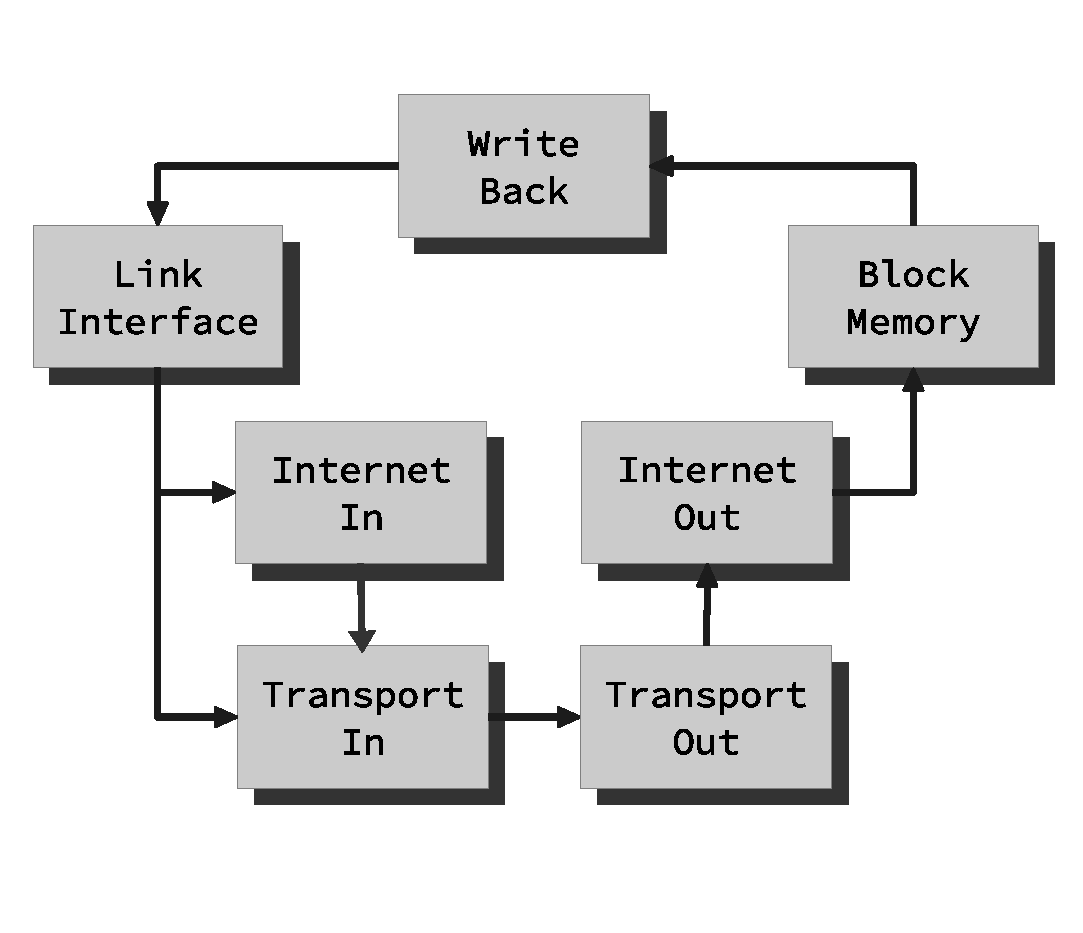
\includegraphics[scale=0.45]{design/design_0.eps}
    \caption{The initial design}
    \label{fig:initial_design}
\end{figure}

The initial architecture focused heavily on the input from the link interface, 
minimizing hardware memory requirements, and to minimize the latency from the 
source data-stream to its respective layer handler.\\
In the initial design, figure \ref{fig:initial_design}, the link interface, which
provides the raw byte-stream from the network, is connected to all of the input
parsing layers. The layers are connected in the order in which a network frame 
is parsed; link- to internet- to transport-layer. This approach aims to utilize
the fact that the layers can act immediatelly upon the packets received directly
from the source, avoid having to buffer the whole packet in each stage, as well 
as easing the logic required to buffer the data across the layers.\\
This design starts by the Link Interface sending one byte at a time through its bus. 
The \texttt{Link In} will parse the first header, and signal the next layer upon completion.
\texttt{Internet In} will then start to listen on the \texttt{Link Interface} bus
and, using the information from \texttt{Link In}, parse the internet header 
accordingly. The same procedure would be applied to the connection between 
\texttt{Internet In} and \texttt{Transport In}.\\
When data is to be sent to the internet, the network frame would be built bottom
up from the transport layer through internet to the link layer.

\subsubsection{The issues}
The issues quickly surfaced during the implementation of the design. Although 
the interconnect from the \texttt{Link Interface} to all the subsequent layers
in parallel promised negligible latency, it came with a great cost to the solution:
\begin{enumerate}

\item \textbf{Process under-utilization} \label{item:process_utilization}\\
Since each "in" process has to wait for the previous layer to signal when to 
start listening on the data-bus, the layers would in average only be active a third
of the time. Since each layer has very little information about the states of 
the other layers, it would become a challenge to get any other work done during
these phases.\\
For example, it would be an immense challenge to coordinate an ICMP reply on a 
faulty packet in the \texttt{Internet In}.

\item \textbf{Redundant Link layer}\\
While the Link layer is an essential part of the Internet Protocol Suite, it did 
not fit well with the functionality of the rest of the stack. 
Most network interfaces are equipped with buffers, on which integrated circuits
perform operations such as error check using cyclic redundancy check, de-noising,
timeslot management, etc. 
Likewise, the Pmod NIC100 Ethernet interface has built-in controller with 
internal memory suited for buffering the incoming packets\cite{microchip_enc424j600}.
This memory, apart from the cyclic redundancy check, can be used as the initial
step for parsing the packet, and only send the datagram to the stack.


\item \textbf{IPv4 fragmentation and out of order TCP packets}\\
The chaotic nature of internet routing might cause packets to come out of order,
or even get fragmented along the way. Since each layer parses the packet immediatelly
as it is written to the bus, it became a challenge for the layers to figure out 
what to do. On IPv4 fragmentation, if the second half of a dataframe arrived 
first, the Transport header would not be available to the Transport layer. 
Although IPv4 fragmentation is an increasingly rare phenomenon, the network 
design is not able to handle the situation well.  

\cofeAm{0.7}{0.75}{2}{80}{0}


\item \textbf{TCP connection state sharing}\\
With a clear separation between the "in" layers and the "out" layers, the 
Transport block had to be split as well. Unfortunately, unlike the other stateless
layers, the transportl layer actually needs to keep track of the connections and 
their states. On every segment received, the appropriate connection needs to be 
updated accordingly.\\
In the TCP protocol, the connection state changes on both receiving and sending.
In this case, the \texttt{Transport In} and \texttt{Transport Out} have to 
agree on a shared state. As these states can be quite large, and the should 
support multiple connections at once, one large bus containing all the information
is not feasible. To solve this, a negotiation protocol may be introduced, however,
as pointed out in item \ref{item:process_utilization}, the processes are very
limited in their execution time. A negotiation would be very hard to achieve in 
such circumstances.
% \item \textbf{Control and logic flow} \\
% Although the layers take turns to parse the incoming byte-stream, the design 
% handles the whole packets at once.  

\end{enumerate}

While it would be possible to work around these identified issues in code, the 
added complexity would have additional ramifications on the project as a whole.
Upon further analysis of analysis, it is clear that the source of the issues is 
the parallel arrangement of the process blocks.

\section{Pipelined design}
\begin{figure}
    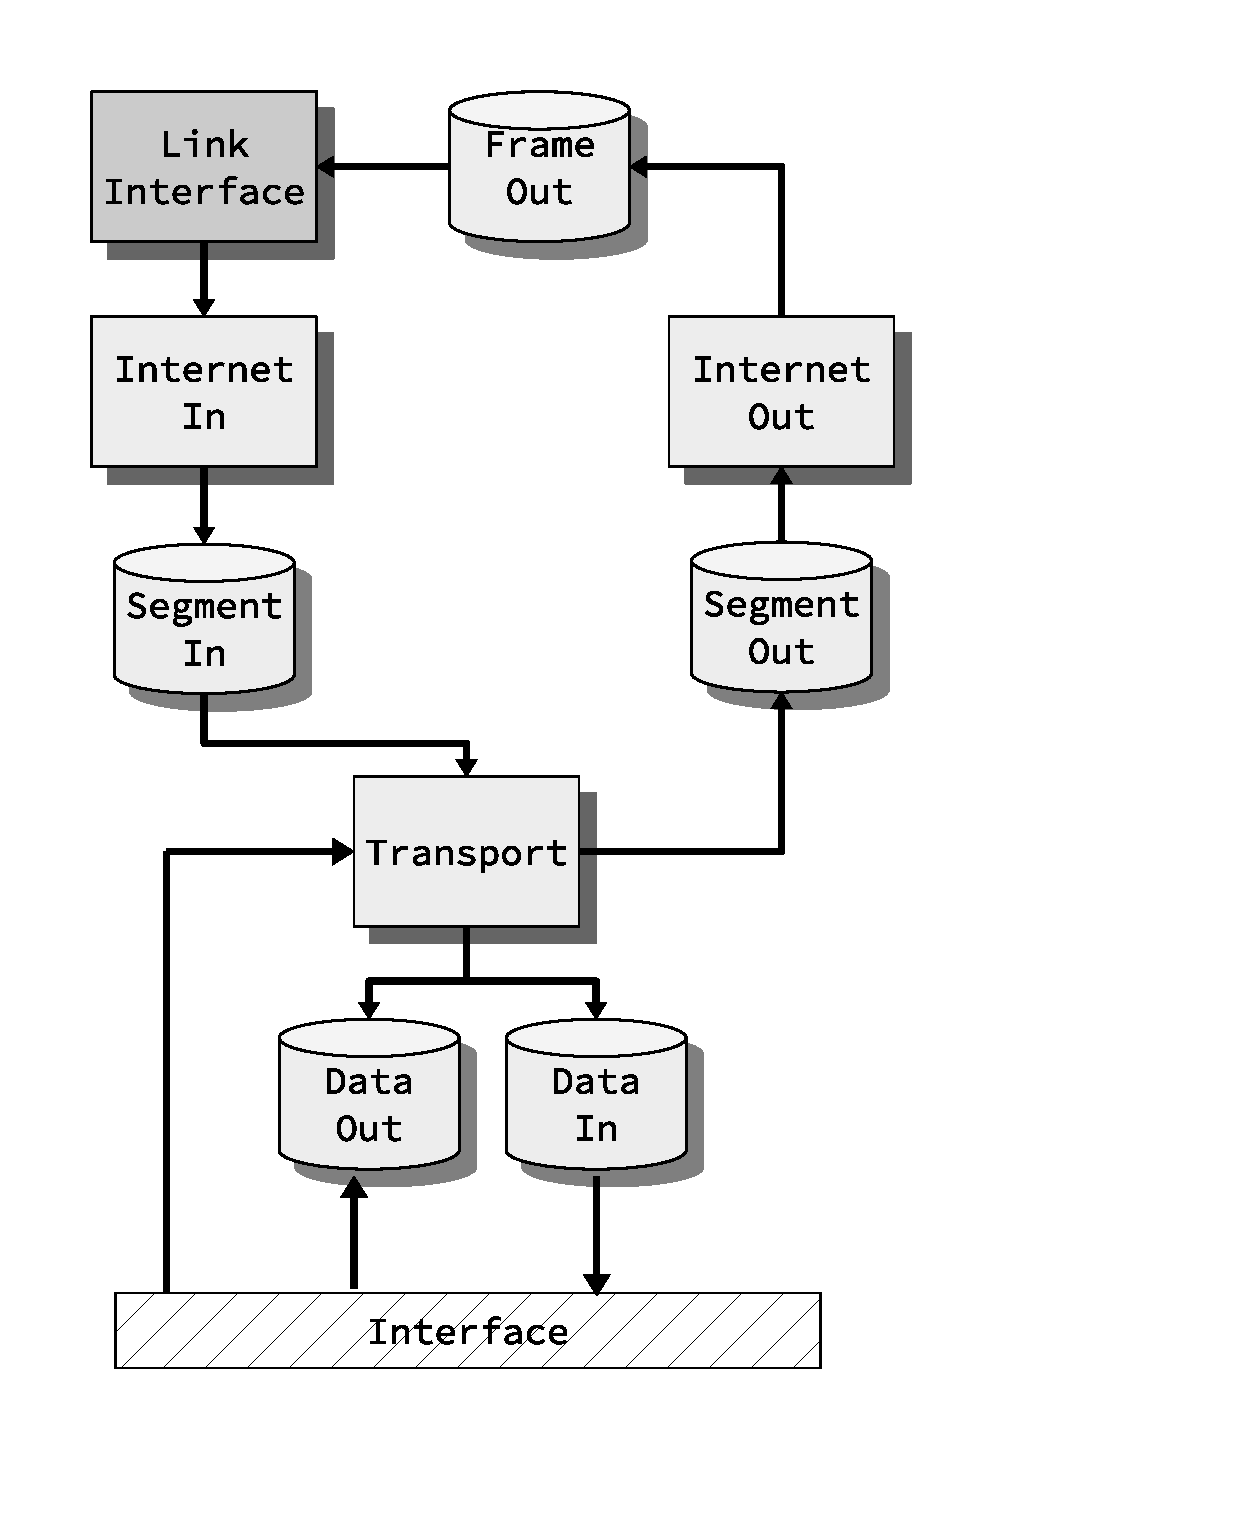
\includegraphics[scale=0.45]{design/design_1.eps}
    \caption{The revised design}
    \label{fig:revised_design}
\end{figure}

The next iteration of the design utilizes a fairly standard approach to 
pipelining, albeit with an unusual transfer of data between the stages.\\
The idea with the pipeline is to enable the processes to receive, compute, and 
forward data at their own pace, without any major limitation from the other 
parts of the system.


\subsection{Internet layer processes} \label{sec:layer_processes}
The processes performing computation and processing on the actual internet 
packets, called "layer processes" for brevity, are by large kept intact from the 
previous design. The fairly simple, but highly sequential nature of packet 
header parsing turned out to be very complicated to optimise with the additional
computing power of the hardware, without introducing too much complication.\\
Missing from the updated figure \ref{fig:revised_design} are the \texttt{Link In}
and \texttt{Link Out} processes, which, for now, are made by the ethernet 
interface, which can easily parse and strip the first frame headers.


\subsection{Data buffers} \label{sec:data_buffers}
Illustrated as cylinders on figure \ref{fig:revised_design}, First-In, First-Out (FIFO)
buffers are introduced between each parsing process in order to control the data-flow 
between the layers. Apart from maintaining a fairly large memory bank through 
the block-RAM, these buffers also contain logic to store the incoming data
intelligently in order to offload the following processes. For example, the
\texttt{Segment In} buffer ensures that fragmented IPv4 packets are defragmented
before leaving the buffer.
However, introducing a new "type" of a process --- the buffers --- poses a new 
challenge. While the buffers can be read from at any time, the layer-parsing
processes do not have this luxury, as they do not have any significant internal
buffer. Hence, a consistent handshake and data-exchange interface signal protocols
are needed.

\subsection{Interface Signal protocols}
With the introduction of buffers between each parsing processes, a clear pattern
emerged. The layer-handling processes are responsible for numerous real-time tasks 
(parsing, sending, protocol-specific tasks, etc), while also limited by their 
fixed internal buffers. These processes are not always ready to receive input 
from preceding processes, while they at the same time must be able to write their
output to following processes immediatelly.\\
The buffers are a stark opposite, as their large internal block memories enable
them to buffer huge chunks of memory, while also being able to wait for the 
succeeding process to start reading.\\
With these two established scenarios, protocols for each can be proposed.  

\subsection{Buffer-Producer data transfer}

\subsection{Compute-Producer data transfer}

% \cofeAm{0.7}{0.75}{2}{80}{0}

